%
% chapter.tex -- Anwendungen von Matrizen in der Codierungstheorie und
%                Kryptographie
%
% (c) 2020 Prof Dr Andreas Müller, Hochschule Rapperswil
%
% !TeX spellcheck = de_CH
\chapter{Anwendungen in Kryptographie
\label{buch:chapter:kryptographie}}
\lhead{Kryptographie}
\rhead{}
Die algebraische Theorie der endlichen Körper hat sich
in der Krypographie als besonders nützliche herausgestellt.
Die Eigenschaften dieser Körper sind reichhaltig genug, um 
kryptographisch widerstandsfähige Algorithmen zu liefern, die
auch in ihrer Stärke beliebig skaliert werden können.
Gleichzeitig liefert die Algebra auch eine effiziente Implementierung.
In diesem Abschnitt soll dies an einigen Beispielen gezeigt werden.

%
% arith.tex
%
% (c) 2021 Prof Dr Andreas Müller, Hochschule Rapperswil
%
\section{Arithmetik für die Kryptographie
\label{buch:section:arithmetik-fuer-kryptographie}}
\rhead{Arithmetik für die Kryptographie}
Die Algorithmen der mathematischen Kryptographie basieren
auf den Rechenoperationen in grossen, aber endlichen Körpern.
Für die Division liefert der euklidische Algorithmus eine
Methode, der in so vielen Schritten die Inverse findet,
wie Dividend und Divisor Binärstellen haben.
Dies ist weitgehend optimal.

Die Division ist umkehrbar, in der Kryptographie strebt man aber an,
Funktionen zu konstruieren, die nur mit grossem Aufwand umkehrbar sind.
Eine solche Funktion ist das Potenzieren in einem endlichen Körper.
Die Berechnung von Potenzen durch wiederholte Multiplikation ist jedoch
prohibitiv aufwendig, daher ist ein schneller Potenzierungsalgorithmus
nötig, der in Abschnitt~\ref{buch:subsection:potenzieren} beschrieben
wird.
Bei der Verschlüsselung grosser Datenmengen wie zum Beispiel bei
der Verschlüsselung ganzer Harddisks mit Hilfe des AES-Algorithmus
kommt es auf die Geschwindigkeit auch der elementarsten Operationen
in den endlichen Körpern an.
Dafür geeignete Methoden werden in den Abschnitten
\ref{buch:subsection:rechenoperationen-in-fp}
und
\ref{buch:subsection:rechenoperatione-in-f2l}
besprochen.

\subsection{Potenzieren
\label{buch:subsection:potenzieren}}
Wir gehen davon aus, dass wir einen schnellen Algorithmus zur
Berechnung des Produktes zweier Elemente $a,b$ in einer
beliebigen Halbgruppe $G$ haben.
Die Halbgruppe $G$ kann die Multiplikation der ganzen oder reellen Zahlen
sein, dies wird zum Beispiel in Implementationen der Potenzfunktion
in Programmierbibliotheken verwendet.
Für kryptographische Anwendungen ist $G$ die multiplikative Gruppe
eines endlichen Körpers oder eine elliptische Kurve
(siehe Abschnitt~\ref{buch:section:elliptische-kurven}).

Zur Berechnung von $a^k$ in $\mathbb{F}_p$ sind bei einer naiven Vorgehensweise
$k-1$ Multiplikationen nötig, immer sofort gefolgt
von einer Reduktion modulo $p$ um sicherzustellen, dass die Resultate
nicht zu gross werden.
Ist $l$ die Anzahl der Binärstellen von $k$, dann benötigt dieser
naive Algorithmus $O(2^l)$ Operationen, die Laufzeit wächst
also exponentiell mit der Bitlänge von $k$ an.
Der nachfolgend beschriebene Algorithmus reduziert die Laufzeit auf
$O(l)$.

Zunächst schreiben wir den Exponenten $k$ in binärer Form als
\[
k = k_l2^l + k_{l-1}2^{l-1} + \dots k_22^2+k_12^1 k_02^0.
\]
Die Potenz $a^k$ kann dann geschrieben werden als
\[
a^k
=
a^{k_l2^l} \cdot a^{k_{l-1}2^{l-1}} \cdot \dots \cdot
a^{k_22^2} \cdot a^{k_12^1} \cdot a^{k_02^0}
\]
Nur diejenigen Faktoren tragen etwas bei, für die $k_i\ne 0$ ist.
Die Potenz kann man daher auch schreiben als
\[
a^k
=
\prod_{k_i\ne 0} a^{2^i}.
\]
Es sind also nur so viele Faktoren zu berücksichtigen, wie $k$ 
Binärstellen $1$ hat.

Die einzelnen Faktoren $a^{2^i}$ können durch wiederholtes Quadrieren
erhalten werden:
\[
a^{2^i} = a^{2\cdot 2^{i-1}} = (a^{2^{i-1}})^2,
\]
also durch maximal $l-1$ Multiplikationen.

Wenn $a\in\mathbb{R}$ und $k$ keine Ganzzahl ist sondern auch noch
binäre Nachkommastellen hat, also
\[
k=k_l2^l + \dots + k_12^1 + k_02^0 + {\color{red}k_{-1}2^{-1} + k_{-2}2^{-2}+\dots,}
\]
dann können die Potenzen ${\color{red}a^{2^{-i}}}$ durch wiederholtes Wurzelziehen
\[
\color{red}
a^{2^{-i}} = a^{\frac12\cdot 2^{-i+1}} = \sqrt{a^{2^{-i+1}}}
\]
gefunden werden.
Die Berechnung der Quadratwurzel lässt sich in Hardware effizient
implementieren.

\begin{algorithmus}
\label{buch:crypto:teile-und-hersche}
Der folgende Algorithmus berechnet $a^k$ in $O(\log_2(k))$
Multiplikationen
\begin{enumerate}
\item Initialisiere $f=1$ und $q=a$
\item Falls $k$ ungerade ist, also $k_i=1$, setze $f:=f\cdot q$ 
\item Setze $q:=q^2$ und $k := k/2$, wobei die ganzzahlige Division durch $2$
am effizientesten als Rechtsshift implementiert werden kann.
\item Falls $k>0$, fahre weiter bei 2.
\end{enumerate}
\end{algorithmus}

\begin{beispiel}
Die Berechnung von $1.1^{17}$ mit diesem Algorithmus ergibt
\begin{enumerate}
\item $f=1$, $q=1.1$
\item $k$ ist ungerade: $f:=1.1$
\item $q:=q^2=1.21$, $k := 8$
\item $k$ ist gerade
\item $q:=q^2=1.4641$, $k := 4$
\item $k$ ist gerade
\item $q:=q^2=2.14358881$, $k := 2$
\item $k$ ist gerade
\item $q:=q^2=4.5949729863572161$, $k := 1$
\item $k$ ist ungerade: $f:=f\cdot q=1.1\cdot p = 5.05447028499293771$
\item $k:=0$
\end{enumerate}
Multiplikationen sind nur nötig in den Schritten 3, 5, 7, 9, 10, es
werden also genau $5$ Multiplikationen ausgeführt statt die
16 Multiplikationen, die bei der naiven Vorgehensweise nötig wären.
\end{beispiel}


\subsection{Rechenoperationen in $\mathbb{F}_p$
\label{buch:subsection:rechenoperationen-in-fp}}
Die Multiplikation macht aus zwei Faktoren $a$ und $b$ ein 
Resultat mit Bitlänge $\log_2 a+\log_2 b$, die Bitlänge wird
also typischerweise ungefähr verdoppelt.
In $\mathbb{F}_p$ muss anschliessend das Resultat modulo $p$
reduziert werden, so dass die Bitlänge wieder höchstens
$\log_2p$ ist.
In folgenden soll gezeigt werden, dass dieser Speicheraufwand 
für eine Binärimplementation deutlich reduziert werden kann,
wenn die Reihenfolge der Operationen modifiziert wird.

\begin{figure}
\begin{center}
\begin{tabular}{>{$}r<{$}>{$}r<{$}>{$}r<{$}|>{$}r<{$}>{$}r<{$}>{$}r<{$}}
\text{Multiplikation mit $2$}&\text{Reduktion?}&\text{reduziert}
	&\text{Summanden}&\text{Summe}&\text{reduziert}
\\
\hline
\texttt{101111}               &                &\texttt{101111} &\texttt{101111}&\texttt{101111}&\texttt{101111}
\\
\texttt{101111\phantom{0}}    &\texttt{{\color{red}1011110}}&\texttt{101001} &               &               &
\\
\texttt{101111\phantom{00}}   &\texttt{{\color{red}1010010}}&\texttt{011101} &               &               &
\\
\texttt{101111\phantom{000}}  &\texttt{0111010}&\texttt{111010} &\texttt{000101}&\texttt{110100}&\texttt{110100}
\\
\texttt{101111\phantom{0000}} &\texttt{\color{red}1110100}&\texttt{111111} &               &               &
\\
\texttt{101111\phantom{00000}}&\texttt{\color{red}1111110}&\texttt{010100} &\texttt{010100}&\texttt{{\color{red}1001000}}&\texttt{10011}\rlap{$\mathstrut=19$}
\end{tabular}
\end{center}
\caption{Multiplikation von $41=\texttt{101001}_2$ mit $47=\texttt{101111}_2$
in $\mathbb{F}_{53}$.
Um die Länge des Resultates zu kontrollieren, wird nach jeder
Multplikation mit $2$ modulo $p=53$ reduziert.
Falls das Resultat
$>p$ ist, wie in den rot markierten Zeilen $p=53=\texttt{110101}_2$
so lange nötig subtrahiert.
Bei der Bildung der Summe wird ebenfalls in jedem Schritt falls nötig
reduziert, angezeigt durch die roten Zahlen in der zweitletzten
Spalte.
Die Anzahl der Subtraktionen, die für die Reduktionen nötig sind, ist
von der selben Grössenordnung wie bei der Durchführung des
Divisionsalgorithmus.
\label{buch:crypto:fig:reduktion}}
\end{figure}

Für die Multiplikation von $41\cdot 47$ rechnet man im Binärsystem
\begin{center}
\begin{tabular}{>{$}r<{$}}
\texttt{{\color{darkgreen}1}0{\color{red}1}001}\cdot\texttt{101111}\\
\hline
\texttt{101111}\\
\texttt{{\color{red}101111}\phantom{000}}\\
\texttt{{\color{darkgreen}101111}\phantom{00000}}\\
\hline
\texttt{11110000111}\\
\hline
\end{tabular}
\end{center}
In $\mathbb{F}_{53}$ muss im Anschluss Modulo $p=53$ reduziert werden.

Der Speicheraufwand entsteht zunächst dadurch, dass durch die Multiplikation
mit $2$ die Summanden immer länger werden.
Man kann den die Sumanden kurz halten, indem man jedesmal, wenn 
der Summand nach der Multiplikation mit $2$ grösser als $p$ geworden ist,
$p$ subtrahiert (Abbildung~\ref{buch:crypto:fig:reduktion}).
Ebenso kann nach jeder Addition des bereits reduzierten zweiten
Faktors wieder reduziert werden.
Die Anzahl der nötigen Reduktionsoperationen wird durch diese
frühzeitig durchgeführten Reduktionen nicht teurer als bei der Durchführung
des Divisionsalgorithmus.


Es ist also möglich, mit gleichem Aufwand an Operationen
aber mit halbem Speicherplatzbedarf die Multiplikationen in $\mathbb{F}_p$
durchzuführen.
Die Platzeinsparung ist besonders bei Implementationen in Hardware 
hilfreich, wo on-die Speicherplatz teuer sein kann.

\begin{figure}
\centering
\includegraphics{chapters/90-crypto/images/schieberegister.pdf}
\caption{Implementation der Multiplikation mit $X$ in einem 
endlichen Körper $\mathbb{F}_{2^l}$ mit dem Minimalpolynom
$m(X) = X^8+X^4+X^3+X^+1$ als Feedback-Schieberegister.
\label{buch:crypto:fig:schieberegister}}
\end{figure}

\subsection{Rechenoperationen in $\mathbb{F}_{2^l}$
\label{buch:subsection:rechenoperatione-in-f2l}}
Von besonderem praktischem Interesse sind die endlichen Körper
$\mathbb{F}_{2^l}$.
Die arithmetischen Operationen in diesen Körpern lassen sich besonders
effizient in Hardware realisieren.

\begin{figure}
\centering
\includegraphics[width=\textwidth]{chapters/90-crypto/images/multiplikation.pdf}
\caption{Multiplikation zweier Elemente von $\mathbb{F}_{2^l}$.
Mit Hilfe des Schieberegisters am linken Rand werden die Produkte 
$X\cdot p(X)$, $X^2\cdot p(X),\dots,X^7\cdot p(X)$ nach der in
Abbildung~\ref{buch:crypto:fig:schieberegister} dargestellten
Methode berechnet.
Am rechten Rand werden diejenigen $X^k\cdot p(X)$ aufaddiert,
für die der $X^k$-Koeffizient von $q(X)$ von $0$ verschieden ist.
\label{buch:crypto:fig:multiplikation}}
\end{figure}

\subsubsection{Zahldarstellung}
Ein endlicher Körper $\mathbb{F}_{2^l}$ ist definiert durch ein
irreduzibles Polynom in $\mathbb{F}_2[X]$ vom Grad $2^l$ 
\[
m(X)
=
X^l + m_{l-1}X^{l-1} + m_{l-2}X^{l-2} + \dots + m_2X^2 + m_1X + m_0
\]
gegeben.
Ein Element in $\mathbb{F}_2[X]/(m)$ kann
durch ein Polynom vom Grad $l-1$
dargestellt werden, also durch
\[
a = a_{l-1}X^{l-1} + a_{l-2}X^{l-2} +\dots + a_2X^2 + a_1X + a_0.
\]
In einer Maschine kann ein Elemente von $\mathbb{F}_2[X]/(m)$
also als eine Bitfolge der Länge $l$
dargestellt werden.


\subsubsection{Addition}
Die Addition in $\mathbb{F}_2$ ist in Hardware besonders leicht zu
realisieren.
Die Addition ist die XOR-Operation, die Multiplikation ist die UND-Verknüfung.
Ausserdem stimmen in $\mathbb{F}_2$ Addition und Subtraktion überein.

Die Addition zweier Polynome erfolgt komponentenweise.
Die Addition von zwei Elemente von $\mathbb{F}_{2^l}$ kann also
durch die bitweise XOR-Verknüpfung der Darstellungen der Summanden 
erfolgen.
Diese Operation ist in einem einzigen Maschinenzyklus realisierbar.
Die Subtraktion, die für die Reduktionsoperation modulo $m(X)$ nötig
ist, ist mit der Addition identisch.


\subsubsection{Multiplikation}
Die Multiplikation zweier Polynome benötigt zunächst die Multiplikation
mit $X$, wodurch der Grad des Polynoms ansteigt und möglicherweise so
gross wird, dass eine Reduktionsoperation modulo $m(X)$ nötig wird.
Die Reduktion wird immer dann nötig, wenn der Koeffizient von $X^l$
nicht $0$ ist.
Der Koeffizient kann dann zum Verschwinden gebracht werden, indem
$m(X)$ addiert wird.

In Abbildung~\ref{buch:crypto:fig:schieberegister} wird gezeigt,
wie die Reduktion erfolgt, wenn die Multiplikation mit $X$, also der
Shift nach links, einen Überlauf ergibt.
Das Minimalpolynom $m(X)=X^8+X^4+X^3+X+1$ bedeutet, dass in $\mathbb{F}_{2^l}$
$X^8=X^4+X^3+X+1$ gilt, so dass man das Überlaufbit durch 
$X^4+X^3+X+1$ ersetzen und addieren kann.

Ein Produkt $p(X)\cdot q(X)$, wobei $p(X)$ und
$q(X)$ Repräsentaten von Elementen $\mathbb{F}_{2^l}$ sind, kann jetzt
wie folgt berechnet werden.
Mit einem Schieberegister werden die Vielfachen $X^k\cdot p(X)$ 
für $k=0,\dots,l-1$ berechnet.
Diejenigen Vielfachen, für die der Koeffizient von $X^k$ in $q(X)$
von $0$ verschieden ist werden aufsummiert und ergeben das Produkt.
Der Prozess in Abbildung~\ref{buch:crypto:fig:multiplikation}
dargestellt.





%
% ff.tex -- Kryptographie und endliche Körper
%
% (c) 2020 Prof Dr Andreas Müller, Hochschule Rapperswil
%

\section{Kryptographie und endliche Körper
\label{buch:section:kryptographie-und-endliche-koerper}}
\rhead{Kryptographie und endliche Körper}
In diesem Abschnitt soll illustriert werden, wie die Arithmetik in
endlichen Körpern Algorithmen zu konstruieren erlaubt, mit denen sich
zum Beispiel sehr effizient kryptographische Schlüssel aushandeln 
lassen.
Der klassische Diffie-Hellmann-Algorithmus in einem Galois-Körper
$\mathbb{F}_p$ wird in Abschnitt~\ref{buch:subsection:elliptische-kurven}
verallgemeinert auf eine sogenannte elliptische Kurve.
Diese Version des Algorithmus ist sehr effizient was die Bitlänge der
Schlüssel betrifft.

\subsection{Potenzen in $\mathbb{F}_p$ und diskreter Logarithmus
\label{buch:subsection:potenzen-diskreter-logarithmus}}
Für kryptographische Anwendungen wird eine einfach zu berechnende
Funktion benötigt,
die ohne zusätzliches Wissen, üblicherweise der Schlüssel genannt,
nicht ohne weiteres umkehrbar ist.
Die arithmetischen Operationen in einem endlichen Körper sind
mit geringem Aufwand durchführbar.
Für die ``schwierigste'' Operation, die Division, steht der
euklidische Algorithmus zur Verfügung.

Die nächstschwierigere Operation ist die Potenzfunktion.
Dank dem Algorithmus~\ref{buch:crypto:teile-und-hersche} ist auch
sie effizient durchführbar.

%Für $g\in \Bbbk$ und $a\in\mathbb{N}$ ist die Potenz $g^a\in\Bbbk$
%natürlich durch die wiederholte Multiplikation definiert.
%In der Praxis werden aber $g$ und $a$ Zahlen mit vielen Binärstellen
%sein, die die wiederholte Multiplikation ist daher sicher nicht
%effizient, das Kriterium der einfachen Berechenbarkeit scheint
%also nicht erfüllt.
%Der folgende Algorithmus berechnet die Potenz in $O(\log_2 a)$
%Multiplikationen.
%
%\begin{algorithmus}[Divide-and-conquer]
%\label{buch:crypto:algo:divide-and-conquer}
%Sei $a=a_0 + a_12^1 + a_22^2 + \dots + a_k2^k$ die Binärdarstellung
%der Zahl $a$.
%\begin{enumerate}
%\item setze $f=g$, $x=1$, $i=0$
%\label{divide-and-conquer-1}
%\item solange $i\ge k$ ist, führe aus
%\label{divide-and-conquer-2}
%\begin{enumerate}
%\item
%\label{divide-and-conquer-3}
%falls $a_i=1$ setze $x \coloneqq x \cdot f$
%\item
%\label{divide-and-conquer-4}
%$i \coloneqq i+1$ und $f\coloneqq f\cdot f$
%\end{enumerate}
%\end{enumerate}
%Die Potenz $x=g^a$ kann so in $O(\log_2a)$ Multiplikationen
%berechnet werden.
%\end{algorithmus}
%
%\begin{proof}[Beweis]
%Die Initalisierung in Schritt~\ref{divide-and-conquer-1} stellt sicher,
%dass $x$ den Wert $g^0$ hat. 
%Schritt~\ref{divide-and-conquer-4} stellt sicher,
%dass die Variable $f$ immer den Wert $g^{2^i}$ hat.
%Im Schritt~\ref{divide-and-conquer-3} wird zu $x$ die Potenz
%$g^{a_i2^i}$ hinzumultipliziert.
%Am Ende des Algorithmus hat daher $x$ den Wert
%\[
%x = g^{a_02^0} \cdot g^{a_12^1} \cdot g^{a_22^2} \cdot\ldots\cdot 2^{a_k2^k}
%=
%g^{a_0+a_12+a_22^2+\dots+a_k2^k}
%=
%g^a.
%\]
%Die Schleife wird $\lfloor1+\log_2ab\rfloor$ mal durchlaufen.
%In jedem Fall wird auf jeden Fall die Multiplikation in 
%Schritt~\ref{divide-and-conquer-4} durchgeführt
%und im schlimmsten Fall auch noch die Multiplikation in
%Schritt~\ref{divide-and-conquer-3}.
%Es werden also nicht mehr als $2\lfloor 1+\log_2a\rfloor=O(\log_2a)$
%Multiplikationen durchgeführt.
%\end{proof}

\begin{beispiel}
Man berechne die Potenz $7^{2021}$ in $\mathbb{F}_p$.
Die Binärdarstellung von 2021 ist $2021_{10}=\texttt{11111100101}_2$.
Wir stellen die nötigen Operationen des
Algorithmus~\ref{buch:crypto:algo:teile-und-hersche} in der folgenden
Tabelle
\begin{center}
\begin{tabular}{|>{$}r<{$}|>{$}r<{$}|>{$}r<{$}|>{$}r<{$}|}
\hline
 i&   q& k_i&    f\\
\hline
 0&   7&   1&    7\\
 1&  49&   0&    7\\
 2&1110&   1&   24\\
 3& 486&   0&   24\\
 4&1234&   0&   24\\
 5& 667&   1&  516\\
 6& 785&   1&  977\\
 7& 418&   1&  430\\
 8& 439&   1&  284\\
 9& 362&   1&  819\\
10& 653&   1&  333\\
\hline
\end{tabular}
\end{center}
In der Spalte $q$ stehen die Potenzen $a^{i+1}=7^{i+1}$, in Spalte $f$ die
ausgerechneten Produkte.
Daraus liest man ab, dass $7^{2021}=333\in\mathbb{F}_{1291}$.
\end{beispiel}

Die Tabelle suggeriert, dass die Potenzen von $g$ ``wild'', also
scheinbar ohne System in $\mathbb{F}_p$ herumspringen.
Dies deutet an, dass die Umkehrung der Exponentialfunktion in $\mathbb{F}_p$
schwierig ist.
Die Umkehrfunktion der Exponentialfunktion, die Umkehrfunktion von 
$x\mapsto g^x$ in $\mathbb{F}_p$ heisst der {\em diskrete Logarithmus}.
\index{diskreter Logarithmus}%
Tatsächlich ist der diskrete Logarithmus ähnlich schwierig zu bestimmen
wie das Faktorisieren von Zahlen, die das Produkt grosser
Primafaktoren ähnlicher Grössenordnung wie $p$ sind.
Die Funktion $x\mapsto g^x$ ist die gesuchte, schwierig zu invertierende
Funktion.

%Auf dern ersten Blick scheint der
%Algorithmus~\ref{buch:crypto:algo:divide-and-conquer}
%den Nachteil zu haben, dass erst die Binärdarstellung der Zahl $a$ 
%ermittelt werden muss.
%In einem Computer ist dies aber normalerweise kein Problem, da $a$
%im Computer ohnehin binär dargestellt ist.
%Die Binärziffern werden in der Reihenfolge vom niederwertigsten zum
%höchstwertigen Bit benötigt.
%Die folgende Modifikation des Algorithmus ermittelt laufend
%auch die Binärstellen von $a$.
%Die dazu notwendigen Operationen sind im Binärsystem besonders
%effizient implementierbar, die Division durch 2 ist ein Bitshift, der
%Rest ist einfach das niederwertigste Bit der Zahl.
%
%\begin{algorithmus}
%\label{buch:crypto:algo:divide-and-conquer2}
%\begin{enumerate}
%\item
%Setze $f=g$, $x=1$, $i=0$
%\item
%Solange $a>0$ ist, führe aus
%\begin{enumerate}
%\item
%Verwende den euklidischen Algorithmus um $r$ und $b$ zu bestimmen mit $a=2b+r$
%\item
%Falls $r=1$ setze $x \coloneqq x \cdot f$
%\item
%$i \coloneqq i+1$, $a = b$ und $f\coloneqq f\cdot f$
%\end{enumerate}
%\end{enumerate}
%Die Potenz $x=g^a$ kann so in $O(\log_2a)$ Multiplikationen
%berechnet werden.
%\end{algorithmus}


%
% Diffie-Hellman Schlüsseltausch
%
\subsection{Diffie-Hellman-Schlüsseltausch
\label{buch:subsection:diffie-hellman}}
Eine Grundaufgabe der Verschlüsselung im Internet ist, dass zwei
Kommunikationspartner einen gemeinsamen Schlüssel für die Verschlüsselung
der Daten aushandeln können müssen.
Es muss davon ausgegangen werden, dass die Kommunikation abgehört wird.
Trotzdem soll es für einen Lauscher nicht möglich sein, den 
ausgehandelten Schlüssel zu ermitteln.

Die beiden Partner $A$ und $B$ einigen sich zunächst auf eine Zahl $g$,
die öffentlich bekannt sein darf.
Weiter erzeugen sie eine zufällige Zahl $a$ und $b$, die sie geheim
halten.
Das Verfahren soll aus diesen beiden Zahlen einen Schlüssel erzeugen,
den beide Partner berechnen können, ohne dass sie $a$ oder $b$ 
übermitteln müssen.
Die beiden Zahlen werden daher auch die privaten Schlüssel genannt.

Die Idee von Diffie und Hellman ist jetzt, die Werte $x=g^a$ und $y=g^b$
zu übertragen.
In $\mathbb{R}$ würden dadurch natürlich dem Lauscher auch $a$ offenbart,
er könnte einfach $a=\log_g x$ berechnen.
Ebenso kann auch $b$ als $b=\log_g y$ erhalten werden, die beiden
privaten Schlüssel wären also nicht mehr privat.
Statt der Potenzfunktion in $\mathbb{R}$ muss also eine Funktion
verwendet werden, die nicht so leicht umgekehrt werden kann.
Die Potenzfunktion in $\mathbb{F}_p$ erfüllt genau diese Eigenschaft.
Die Kommunikationspartner einigen sich also auch noch auf die (grosse)
Primzahl $p$ und übermitteln $x=g^a\in\mathbb{F}_p$ und
$y=g^b\in\mathbb{F}_p$.

\begin{figure}
\centering
\includegraphics{chapters/90-crypto/images/dh.pdf}
\caption{Schlüsselaustausch nach Diffie-Hellman.
\index{Diffie-Hellmann}%
\index{Schlüsseltausch}%
Die Kommunikationspartner $A$ und $B$ einigen sich öffentlich auf
$p\in\mathbb{N}$ und $g\in\mathbb{F}_p$.
$A$ wählt dann einen privaten Schlüssel $a\in\mathbb{N}$ und
$B$ wählt $b\in\mathbb{N}$, sie tauschen dann $x=g^a$ und $y=g^b$
aus.
$A$ erhält den gemeinsamen Schlüssel aus $y^a$, $B$ erhält ihn
aus $x^b$.
\label{buch:crypto:fig:dh}}
\end{figure}

Aus $x$ und $y$ muss jetzt der gemeinsame Schlüssel abgeleitet werden.
$A$ kennt $y=g^b$ und $a$, $B$ kennt $x=g^a$ und $b$.
Beide können die Zahl $s=g^{ab}\in\mathbb{F}_p$ berechnen.
$A$ macht das, indem er $y^a=(g^b)^a = g^{ab}$ rechnet,
$B$ rechnet $x^b = (g^a)^b = g^{ab}$, beide natürlich in $\mathbb{F}_p$.
Der Lauscher kann aber $g^{ab}$ nicht ermitteln, dazu müsste er
$a$ oder $b$ ermitteln können.
Die Zahl $s=g^{ab}$ kann also als gemeinsamer Schlüssel verwendet
werden.


%
% elliptisch.tex
%
% (c) 2021 Prof Dr Andreas Müller, OST Ostshweizer Fachhochschule
%
\section{Elliptische Kurven
\label{buch:section:elliptische-kurven}}
\index{elliptische Kurve}%
\rhead{Elliptische Kurven}
Das Diffie-Hellman-Verfahren basiert auf der Schwierigkeit, in einem 
Körper $\mathbb{F}_p$ die Gleichung $a^x=b$ nach $x$ aufzulösen.
Die Addition in $\mathbb{F}_p$ wird dazu nicht benötigt.
Es reicht, eine Menge mit einer Multiplikation zu haben, fir die
die Gleichung $a^x=b$ schwierig nach $x$ aufzulösen ist.
Ein Halbgruppe wäre also durchaus ausreichend.

Ein Kandidat für eine solche Gruppe könnte der Einheitskreis
$S^1=\{z\in\mathbb{C} \mid |z|=1\}$ in der komplexen Ebene sein.
Wählt man eine Zahl $g=e^{i\alpha}$, wobei $\alpha$ ein irrationales
Vielfaches von $\pi$ ist, dann sind alle Potenzen $g^n$ für natürliche
Exponenten voneinander verschieden.
Wäre nämlich $g^{n_1}=g^{n_2}$, dann wäre $e^{i\alpha(n_1-n_2)}=1$ und
somit müsste $\alpha=2k\pi/(n_1-n_2)$ sein.
Damit wäre aber $\alpha$ ein rationales Vielfaches von $\pi$, im Widerspruch
zur Voraussetzung.
Die Abbildung $n\mapsto g^n\in S^1$ ist auf den ersten Blick etwa ähnlich
undurchschaubar wie die Abbildung $n\mapsto g^n\in\mathbb{F}_p$.
Es gibt zwar die komplexe Logarithmusfunktion, mit der man $n$ bestimmen
kann, dazu muss man aber den Wert von $g^n$ mit beliebiger Genauigkeit
kennen, denn die Werte von $g^n$ können beliebig nahe beieinander liegen.

Der Einheitskreis ist die Lösungsmenge der Gleichung $x^2+y^2=1$ für
reelle Koordinaten $x$ und $y$,
doch Rundungsunsicherheiten verunmöglichen den Einsatz in einem 
Verfahren ähnlich dem Diffie-Hellman-Verfahren.
Dieses Problem kann gelöst werden, indem für die Variablen Werte
aus einem endlichen Körper verwendet werden.
Gesucht ist also eine Gleichung in zwei Variablen, deren Lösungsmenge
in einem endlichen Körper eine Gruppenstruktur trägt.
Die Lösungsmenge ist eine ``Kurve'' von Punkten mit
\index{Kurve}%
Koordinaten in einem endlichen Körper.

In diesem Abschnitt wird gezeigt, dass sogenannte elliptische Kurven
über endlichen Körpern genau die verlangten Eigenschaften haben.

\subsection{Definition}
Elliptische Kurven sind Lösungen einer Gleichung der Form
\begin{equation}
Y^2+XY=X^3+aX+b
\label{buch:crypto:eqn:ellipticcurve}
\end{equation}
mit Werten von $X$ und $Y$ in einem geeigneten Körper.
Die Koeffizienten $a$ und $b$ müssen so gewählt werden, dass die
Gleichung~\eqref{buch:crypto:eqn:ellipticcurve} genügend viele
Lösungen hat.
Über den komplexen Zahlen hat die Gleichung natürlich für jede Wahl von
$X$ drei Lösungen.
Für einen endlichen Körper können wir dies im allgemeinen nicht erwarten,
aber wenn wir genügend viele Wurzeln zu $\mathbb{F}$ hinzufügen können wir
mindestens erreichen, dass die Lösungsmenge so viele Elemente hat, 
dass ein Versuch, die Gleichung $g^x=b$ mittels Durchprobierens zu
lösen, zum Scheitern verurteilt ist.

\begin{definition}
\label{buch:crypto:def:ellipticcurve}
Die {\em elliptische Kurve} $E_{a,b}(\Bbbk)$ über dem Körper $\Bbbk$ ist 
\index{elliptische Kurve}%
die Menge
\[
E_{a,b}(\Bbbk)
=
\{(X,Y)\in\Bbbk^2 \mid Y^2+XY=X^3+aX+b\},
\]
für $a,b\in\Bbbk$.
\end{definition}

\subsection{Visualisierung über dem Körper $\mathbb{R}$}
Um die Anschauung zu vereinfachen, werden wir elliptische Kurven über
dem Körper $\mathbb{R}$ visualisieren.
Die daraus gewonnenen geometrischen Einsichten werden wir anschliessend
algebraisch umsetzen.
In den reellen Zahlen kann man die
Gleichung~\eqref{buch:crypto:eqn:ellipticcurve}
noch etwas vereinfachen.
Indem man in \eqref{buch:crypto:eqn:ellipticcurve} 
quadratisch ergänzt, bekommt man
\begin{align}
Y^2 + XY + \frac14X^2 &= X^3+\frac14 X^2 +aX+b
\notag
\\
\Rightarrow\qquad
v^2&=X^3+\frac14X^2+aX+b,
\label{buch:crypto:eqn:ell2}
\end{align}
indem man $v=Y+\frac12X$ setzt.
Man beachte, dass man diese Substition nur machen kann, wenn $\frac12$
definiert ist.
In $\mathbb{R}$ ist dies kein Problem, aber genau über den Körpern
mit Charakteristik $2$, die wir für die Computer-Implementation
bevorzugen, ist dies nicht möglich.
Es geht hier aber nur um die Visualisierung.

Auch die Form \eqref{buch:crypto:eqn:ell2} lässt sich noch etwas 
vereinfachen.
Setzt man $X=u-\frac1{12}$, dann verschwindet nach einiger Rechnung,
die wir hier nicht durchführen wollen, der quadratische Term
auf der rechten Seite.
Die interessierenden Punkte sind Lösungen der einfacheren Gleichung
\begin{equation}
v^2
=
u^3+\biggl(a-\frac{1}{48}\biggr)u + b-\frac{a}{12}+\frac{1}{864}
=
u^3+Au+B.
\label{buch:crypto:ellvereinfacht}
\end{equation}
In dieser Form ist mit $(u,v)$ immer auch $(u,-v)$ eine Lösung,
die Kurve ist symmetrisch bezüglich der $u$-Achse.
Ebenso kann man ablesen, dass nur diejenigen $u$-Werte möglich sind,
für die das kubische Polynom $u^3+Au+B$ auf der rechten Seite von
\eqref{buch:crypto:ellvereinfacht}
nicht negativ ist.

Sind $u_1$, $u_2$ und $u_3$ die Nullstellen des kubischen Polynoms
auf der rechten Seite von~\eqref{buch:crypto:ellvereinfacht}, folgt
\[
v^2
=
(u-u_1)(u-u_2)(u-u_3)
=
u^3
-(u_1+u_2+u_3)u^2
+(u_1u_2+u_1u_3+u_2u_3)u
-
u_1u_2u_3.
\]
Durch Koeffizientenvergleich sieht man, dass $u_1+u_2+u_3=0$ sein muss.
\begin{figure}
\centering
\includegraphics{chapters/90-crypto/images/elliptic.pdf}
\caption{Elliptische Kurve in $\mathbb{R}$ in der Form
$v^2=u^3+Au+B$ mit Nullstellen $u_1$, $u_2$ und $u_3$ des
kubischen Polynoms auf der rechten Seite.
Die blauen Punkte und Geraden illustrieren die Definition der
Gruppenoperation in der elliptischen Kurve.
\label{buch:crypto:fig:elliptischekurve}}
\end{figure}
Abbildung~\ref{buch:crypto:fig:elliptischekurve}
zeigt eine elliptische Kurve in der Ebene $\mathbb{R}^2$.

\subsection{Geometrische Definition der Gruppenoperation}
In der speziellen Form \eqref{buch:crypto:ellvereinfacht} ist die
elliptische Kurve symmetrisch unter Spiegelung an der $u$-Achse.
Die Spiegelung ist eine Involution, zweimalige Ausführung führt auf
den ursprünglichen Punkt zurück.
Die Inverse in einer Gruppe hat diese Eigenschaft auch, es ist
daher naheliegend, den gespiegelten Punkt als die Inverse eines
Elementes zu nehmen.

Eine Gerade durch zwei Punkte der
in Abbildung~\ref{buch:crypto:fig:elliptischekurve}
dargestellten Kurve schneidet die Kurve ein drittes Mal.
Die Gruppenoperation wird so definiert, dass drei Punkte der Kurve
auf einer Geraden das Gruppenprodukt $e$ haben.
Da aus $g_1g_2g_3=e$ folgt $g_3=(g_1g_2)^{-1}$ oder
$g_1g_2=g_3^{-1}$, erhält man das Gruppenprodukt zweier Elemente
auf der elliptischen Kurve indem man erst den dritten Schnittpunkt
ermittelt und diesen dann an der $u$-Achse spiegelt.

Die geometrische Konstruktion schlägt fehl, wenn $g_1=g_2$ ist.
In diesem Fall kann man die Tangente im Punkt $g_1$ an die Kurve 
verwenden.
Dieser Fall tritt zum Beispiel auch in den drei Punkten 
$(u_1,0)$, $(u_2,0)$ und $(u_3,0)$ ein.

Um das neutrale Element der Gruppe zu finden, können wir 
zwei Punkte $g$ und $g^{-1}$ miteinander verknüpfen.
Die Gerade durch $g$ und $g^{-1}$ schneidet aber die Kurve
kein drittes Mal.
Ausserdem sind alle Geraden durch $g$ und $g^{-1}$ für verschiedene
$g$ parallel.
Das neutrale Element entspricht also einem unendlich weit entfernten Punkt.
Das neutrale Element entsteht immer dann als Produkt, wenn zwei
Punkte die gleiche $u$-Koordinaten haben.

\subsection{Gruppenoperation, algebraische Konstruktion}
Nach den geometrischen Vorarbeiten zur Definition der Gruppenoperation
können wir jetzt die Konstruktion algebraisch über einem 
beliebigen Körper umsetzen.

Wir gehen wieder von der elliptischen Kurve in der Form
\begin{equation}
Y^2+XY=X^3+aX+b
\label{buch:crypto:eqn:grupopgl}
\end{equation}
aus.
Man kann dies auch mit dem Polynom mit zwei Variablen
\[
P(X,Y) = Y^2+XY -X^3-aX-b
\]
schreiben.
Ein Punkt $g=(x,y)$ auf der elliptischen Kurve erfüllt die
Bedingung $P(x,y)=0$.

\subsubsection{Involution}
Zunächst überlegen wir uns wieder eine Involution, welche als Inverse
dienen kann.
Dazu beachten wir, dass die linke Seite der definierenden Gleichung
\eqref{buch:crypto:eqn:grupopgl}
auch als $Y(Y+X)$ geschrieben werden kann.
Die Abbildung $Y\mapsto -X-Y$ macht daraus
\[
(-X-Y)(-X-Y+X)=(X+Y)Y.
\]
Mit dem Punkt $(X,Y)$ ist automatisch auch $(X,-X-Y)$
ein Punkt der elliptischen Kurve.
Dies ist die gesuchte Involution.

\subsubsection{Gerade durch zwei Punkte}
Seien also $g_1=(x_1,y_1)$ und $g_2=(x_2,y_2)$ zwei verschiedene Lösungen
der Gleichung \eqref{buch:crypto:eqn:grupopgl}
Als erstes brauchen wir eine Gleichung für die Gerade durch die beiden
Punkte.
Sei also $l(X,Y)$ eine Linearform derart, dass $l(g_1)=d$ und $l(g_2)=d$
für ein geeignetes $d\in\Bbbk$.
Dann gilt auch für die Punkte
\[
g(t) = tg_1 + (1-t)g_2
\qquad\Rightarrow\qquad
l(g(t))
=
tl(g_1) + (1-t)l(g_2)
=
td+(1-t)d
=
(t+1-t)d
=d.
\]
Jeder Punkt $g$ der Geraden durch $g_1$ und $g_2$ erfüllt einerseits
$l(g)=d$, andererseits lässt er sich in dieser Form schreiben $g(t)$
für ein geeignetes $t\in\Bbbk$ schreiben.

\subsubsection{Dritter Schnittpunkt}
Setzt man jetzt $g(t)$ in die Gleichung~\eqref{buch:crypto:eqn:grupopgl}
ein, erhält man eine kubische
Gleichung in $t$, von der wir bereits zwei Nullstellen kennen, nämlich 
$0$ und $1$.
Die kubische Gleichung muss also durch $t$ und $(t-1)$ teilbar sein.
Diese Berechnung kann man einfach in einem Computeralgebrasystem
durchführen.
Das Polynom ist
\begin{align*}
p(t)
&=
(t-1)^2y_2^2
+
((2t-2t^2) y_1 +(t^2-2t+1)x_2 + (t-t^2)x_1)y_2
+
t^2y_1^2
+
((t-t^2)x_2+t^2 x_1)y_1
\\
&\qquad
+
(t^3-3t^2+3t-1)x_2^3
+
(-3 t^3+6t^2-3t)x_1x_2^2
+
((3t^3-3t^2)x_1^2+at-a)x_2
-
t^3x_1^3
-
atx_1-b
\end{align*}
Da die Punkte $g_1=g(0)$ und $g_2=g(1)$ auf der elliptischen Kurve
liegen, muss das Polynom durch die Nullstellen $t=0$ und $t=1$
haben, es muss also durch $t(t-1)$ teilbar sein.
Teilt man durch $t(t-1)$ bleibt ein Polynom ersten Grades mit
einer einzigen Nullstelle, dem dritten Punkt.
Nach Division durch $t(t-1)$ erhält man als Quotienten
\begin{align}
q(t)
&=
(y_2-y_1)^2 
+
(y_2-y_1) (x_2-x_1)
+
t(x_2-x_1)^3
-
2x_2^3+3x_1x_2^2-x_1^3
\label{buch:ecc:eqn:q(t)}
\end{align}
und den Rest
\begin{align*}
r(t)
&=
t(y_1^2+x_1y_1-x_1^3-ax_1-b)
+
(1-t)(y_2^2+x_2y_2-x_2^3-ax_2-b)
\\
&=
tP(x_1,y_1)
+
(1-t)P(x_2,y_2)
=
0.
\end{align*}
Die Klammerausdrücke verschwinden, da sie gleichbedeutend damit sind,
dass die Punkte Lösungen von \eqref{buch:crypto:eqn:grupopgl} sind.
Dies bestätigt nochmals, dass der Rest $r(t)=0$ ist, dass $p(t)$
also durch $t(1-t)$ teilbar ist.

Für den dritten Punkt auf der Geraden muss $t$ so gewählt werden, dass
$q(t)=0$ ist.
Dies ist aber eine lineare Gleichung mit der Lösung
\begin{align*}
t
&=
-\frac{
(y_1-y_2)^2
+
(y_2-y_1)(x_2-x_1)
-2x_2^3+3x_1x_2^2-x_1^3
}{(x_2-x_1)^3}
.
\end{align*}
Setzt man dies $g(t)$ ein, erhält man für die Koordinaten des dritten
Punktes $g_3$ die Werte
\begin{align}
x_3
&=
\frac{
(y_2-y_1)^2(x_2-x_1) + (y_2-y_1)(x_2-x_1)^2
-(x_2^4+x_1^4)
}{
(x_2-x_1)^3
}
\label{buch:crypto:eqn:x3}
\\
y_3
&=
\frac{
(y_2-y_1)^3
+(x_2-x_1)(y_2-y_1)^2
-(x_{2}-x_{1})^3 ( y_{2} - y_{1})
-(x_{2}-x_{1})^2 ( x_{1} y_{2}- x_{2} y_{1})
}{
(x_2-x_1)^3
}
\label{buch:crypto:eqn:y3}
\end{align}
Die Gleichungen 
\eqref{buch:crypto:eqn:x3}
und
\eqref{buch:crypto:eqn:y3}
ermöglichen also, das Element $g_1g_2^{-1}$ zu berechnen.
Interessant daran ist, dass in den Formeln die Konstanten $a$ und $b$ 
gar nicht vorkommen.

\subsubsection{Quadrieren}
Es bleibt noch der für den Algorithmus~\ref{buch:crypto:teile-und-hersche}
wichtige Fall des Quadrierens in der Gruppe zu
behandeln, also der Fall $g_1=g_2$.
In diese Fall sind die Formeln
\eqref{buch:crypto:eqn:x3}
und
\eqref{buch:crypto:eqn:y3}
ganz offensichtlich nicht anwendbar.
Die geometrische Anschauung hat nahegelegt, die Tangent an die Kurve
im Punkt $g_1$ zu nehmen.
In $\mathbb{R}$ würde man dafür einen Grenzübergang $g_2\to g_1$ machen,
aber in einem endlichen Körper ist dies natürlich nicht möglich.

Wir schreiben die Gerade als Parameterdarstellung in der Form
\(
t\mapsto g(t)= (x_1+ut, y_1+vt)
\)
für beliebige Parameter in $\Bbbk$.
Die Werte $u$ und $v$ müssen so gewählt werden, dass $g(t)$ eine
Tangente wird.
Setzt man $g(t)$ in die Gleichung~\eqref{buch:crypto:eqn:grupopgl} ein,
entsteht ein kubische Gleichung, die genau dann eine doppelte Nullstelle
bei $0$ hat, wenn $u,v$ die Tangentenrichtung beschreiben.
Einsetzen von $g(t)$ in \eqref{buch:crypto:eqn:grupopgl}
ergibt die Gleichung
\begin{align}
0
&=
-u^3t^3
+
(-3u^2x_{1}+v^2+uv)t^2
+
(2vy_1+uy_1-3ux_1^2+vx_1-au)t
+
(y_1^2+x_1y_1-x_1^3-ax_1-b)
\label{buch:crypto:eqn:tangente1}
\end{align}
Damit bei $t=0$ eine doppelte Nullstelle müssen die letzten beiden
Koeffizienten verschwinden, dies führt auf die Gleichungen
\begin{align}
y_1^2+x_1y_1&=x_1^3+ax_1+b
\label{buch:crypto:eqn:rest1}
\\
(2y_1
+x_1)v
+(y_1
-3x_1^2
-a)u
&=0.
\label{buch:crypto:eqn:rest2}
\end{align}
Die erste Gleichung \eqref{buch:crypto:eqn:rest1} drückt aus,
dass $g_1$ ein Punkt der Kurve ist, sie ist automatisch erfüllt.

Die zweite Gleichung
\eqref{buch:crypto:eqn:rest2}
legt das Verhältnis von $u$ und $v$, also die
Tangentenrichtung, fest.
Eine mögliche Lösung ist
\begin{equation}
\begin{aligned}
u &= x_1+2y_1
\\
v &= -y_1+3x_1^2+a.
\end{aligned}
\label{buch:crypto:eqn:uv}
\end{equation}

Der Quotient ist ein lineares Polynom in $t$, die Nullstelle parametrisiert
den Punkt, der $(g_1)^{-2}$ entspricht.
Der zugehörige Wert von $t$ ist
\begin{equation}
t=-\frac{3u^2x_1-v^2-uv}{u^3}.
\label{buch:crypto:eqn:t}
\end{equation}


Setzt man
\label{buch:crypto:eqn:t}
und
\eqref{buch:crypto:eqn:uv}
in $g(t)$ ein, erhält man sehr komplizierte Ausdrücke für den dritten Punkt.
Wir verzichten darauf, diese Ausdrücke hier aufzuschreiben.
In der Praxis wird man in einem Körper der Charakteristik 2 arbeiten.
In diesem Körper werden alle geraden Koeffizienten zu $0$, alle ungeraden
Koeffizienten werden unabhängig vom Vorzeichen zu $1$.
Damit bekommt man die folgenden, sehr viel übersichtlicheren Ausdrücke
für den dritten Punkt:
\begin{equation}
\begin{aligned}
x
&=
-\frac{
y_1^2+x_1y_1+x_1^4+x_1^3+ax_1-a^2
 }{
x_1^2
}
\\
y
&=
\frac{
y_1^3+(x_1^2+x_1+a)y_1^2+(x_1^4 +a^2)y_1+x_1^6+ax_1^4+ax_1^3+a^2x_1^2+a^2x_1+a^3
}{
 x_1^3
}.
\end{aligned}
\label{buch:crypto:eqn:tangentechar2}
\end{equation}
Damit haben wir einen vollständigen Formelsatz für die Berechnung der
Gruppenoperation in der elliptischen Kurve mindestens für den praktisch
relevanten Fall einer Kurve über einem Körper der Charakteristik $2$.

\subsubsection{Neutrales Element}
Das neutrale Element erhält man, wenn man das Produkt zweier Punkte
bildet, die durch die Involution auseinander hervorgehen.
Sie haben die gleiche $x$-Koordinate, also $x_1=x_2$.
Im Polynom $q(t)$ von \eqref{buch:ecc:eqn:q(t)} kommt dann aber an
der Stelle $0$ als Koeffizient von $t$ vor.
Das Polynom wird zu $q(t) = (y_2-y_1)^2$, es hat also keine weitere
Nullstelle.
Es scheint also in diesem Fall gar keinen dritten Punkt zu geben.
Ein neutrales Element kann daher nicht die Form eines Punktes $(x,y)$
haben, welcher $P(x,y)=0$ erfüllt.
In der Tat muss man die $\Bbbk^2$-Ebene durch einen Punkt im ``Unendlichen''
erweitern.

Für unsere Zwecke, nämlich für die Konstruktion eines
Diffie-Hellmann-ähnlichen Verfahrens, wird das neutrale Element
nicht wirklich benötigt.
Um den Potenz-Algorithmus~\ref{buch:crypto:teile-und-hersche}
durchzuführen, brauchen wir nur die beiden Operationen
Multiplizieren und Quadrieren, für die wir bereits
geeignete Formeln gefunden haben.

\subsubsection{Gruppenstruktur auf einer elliptischen Kurve}

\begin{satz}
Die elliptische Kurve
\[
E_{a,b}(\mathbb{F}_{p^l})
=
\{
(X,Y)\in\mathbb{F}_{p^l}
\mid
Y^2+XY = X^3-aX-b
\}
\]
trägt eine Gruppenstruktur, die wie folgt definiert ist:
\begin{enumerate}
\item Es gibt ein neutrales Element, welches man manchmal als $(0,0)$
schreibt, obwohl dieser Punkt nicht auf der Kuve liegt.
\item Das inverse Element von $(x,y)$ ist $(x,-y-x)$.
\item Für zwei verschiedene Punkte $g_1$ und $g_2$ kann $g_3=(g_1g_2)^{-1}$
mit Hilfe der Formeln
\eqref{buch:crypto:eqn:x3}
und
\eqref{buch:crypto:eqn:y3}
gefunden werden.
\item Für einen Punkt $g_1$ kann $g_3=g_1^{-2}$ in Charakteristik $2$ mit
Hilfe der Formeln
\eqref{buch:crypto:eqn:tangentechar2}
gefunden werden.
\end{enumerate}
Diese Operationen machen $E_{a,b}(\mathbb{F}_{p^l})$ zu einer endlichen
abelschen Gruppe.
\end{satz}

\subsection{Diffie-Hellman in einer elliptischen Kurve}
Der klassische Diffie-Hellmann-Schlüsselalgorithmus in einem Körper
$\mathbb{F}_p$ basiert darauf, dass man beliebige Potenzen eines 
Elementes berechnen kann, und dass es schwierig ist, diese Operation
umzukehren.
Die Addition in $\mathbb{F}_p$ wird für diesen Algorithmus überhaupt
nicht benötigt.

In einer elliptischen Kurve gibt es ebenfalls eine Multiplikation,
für die sich mit Algorithmus~\ref{buch:crypto:teile-und-hersche}
eine effizienter Potenzieralgorithmus konstruieren lässt.
Die resultierende Potenzfunktion stellt sich ebenfalls als 
schwierig zu invertieren heraus, kann also ebenfalls für einen
Diffie-Hellmann-Schlüsseltausch verwendet werden.

Die im Internet Key Exchange Protokol
in RFC 2409
\cite{buch:rfc2409}
definierte Oakley-Gruppe 4
zum Beispiel verwendet einen Galois-Körper $\mathbb{F}_{2^{185}}$ 
mit dem Minimalpolynom $m(x)=x^{185}+x^{69}+1\in \mathbb{F}_2[x]$
und den Koeffizienten
\begin{align*}
a&=0\\
b&=x^{12}+x^{11} + x^{10} + x^9 + x^7 + x^6 + x^5 + x^3 +1,
\end{align*} 
die die elliptische Kurve definieren.

Als Elemente $g$ für den Diffie-Hellmann-Algorithmus wird ein Punkt
der elliptischen Kurve verwendet, dessen $X$-Koordinaten durch das
Polynom $g(x) = x^4+x^3$ gegeben ist.
Der Standard spezifiziert die $Y$-Koordinate nicht, diese kann aus
den gegebenen Daten abgeleitet werden.
Die entstehende Gruppe hat etwa $4.9040\cdot10^{55}$ Elemente, die
für einen brute-force-Angriff durchprobiert werden müssten.









%
% aes.tex -- Beschreibung des AES Algorithmus
%
% (c) 2020 Prof Dr Andreas Müller, Hochschule Rapperswil
%
\section{Advanced Encryption Standard -- AES
\label{buch:section:aes}}
\rhead{Advanced Encryption Standard}
Eine wichtige Forderung bei der Konzeption des damals neuen
Advanced Encryption Standard war, dass darin keine ``willkürlich''
erscheinenden Operationen geben darf, bei denen der Verdacht
entstehen könnte, dass sich dahinter nicht offengelegtes Wissen
über einen möglichen Angriff auf den Verschlüsselungsalgorithmus
verbergen könnte.
Dies war eine Schwäche des vor AES üblichen DES Verschlüsselungsalgorithmus.
In seiner Definition kommt eine Reihe von Konstanten vor, über deren
Herkunft nichts bekannt war.
Die Gerüchteküche wollte wissen, dass die NSA die Konstanten aus dem
ursprünglichen Vorschlag abgeändert habe, und dass dies geschehen sei,
um den Algorithmus durch die NSA angreifbar zu machen.

Eine weiter Forderung war, dass die Sicherheit des neuen
Verschlüsselungsstandards ``skalierbar'' sein soll, dass man also
die Schlüssellänge mit der Zeit von 128~Bit auf 196 oder sogar 256~Bit
steigern kann.
Der Standard wird dadurch langlebiger und gleichzeitig entsteht die
Möglichkeit, Sicherheit gegen Rechenleistung einzutauschen.
Weniger leistungsfähige Systeme können den Algorithmus immer noch
nutzen, entweder mit geringerer Verschlüsselungsrate oder geringerer
Sicherheit.

In diesem Abschnitt soll gezeigt werde, wie sich die im AES
spezifizierten Operationen mit der Arithmetik 
eines endlichen Körpers beschreiben lassen.
Im Abschnitt~\ref{buch:subsection:byte-operationen} werden
Bytes als Elemente in einem endlichen Körper $\mathbb{F}_{2^8}$
interpretiert.
Damit kann dann die sogenannte $S$-Box konstruiert werden und
es ist leicht zu verstehen, dass sie invertierbar ist.
Aus den Byte-Operationen können dann Mischoperationen erzeugt
werden, die Bytes untereinander verknüpfen, die aber auch wieder
als Operationen in einem endlichen Körper verstanden werden können.

\subsection{Byte-Operationen
\label{buch:subsection:byte-operationen}}
Moderne Prozessoren operieren auf Wörtern, die Vielfache von Bytes sind.
Byte-Operationen sind besonders effizient in Hardware zu realisieren.
AES verwendet daher als Grundelemente Operationen auf Bytes, die als
Elemente eines endlichen Körpers $\mathbb{F}_{2^8}$ interpretiert werden.

\subsubsection{Bytes als Elemente von $\mathbb{F}_{2^8}$}
Das Polynom $m(X)=X^8+X^4+X^3+X+1\in \mathbb{F}_2[X]$ ist irreduzibel,
somit ist $\mathbb{F}_{2^8} = \mathbb{F}_2[X]/(m)$ ein Körper.
Die Elemente können dargestellt werden als Polynome
\[
p(X) = p_7X^7 + p_6X^6 + \dots + p_2X^2+p_1X + p_0,
\]
sie bestehen daher aus den $8$ Bits $p_7,\dots,p_0$.
Das Byte $\texttt{63}_{16}$ entspricht also dem Polynom
$X^6+X^5+X+1$ in $\mathbb{F}_2[X]/(m)$.

Die Interpretation der Bytes als Elemente eines Körpers bedeutet,
dass jede Multiplikation mit einem nicht verschwindenden Byte 
invertierbar ist.
Ausserdem mischen diese Operationen die einzelnen Bits auf einigermassen
undurchsichtige, aber umkehrbare Art durcheinander, wie dies für ein
Verschlüsselungsverfahren wünschenswert ist.

\subsubsection{$S$-Box}
Für die Operation der sogenannten $S$-Box wird wie folgt zusammengesetzt.
Zunächst wird ein Byte $x$ durch das zugehörige multiplikative
inverse Element
\[
x\mapsto \bar{x} = \begin{cases}
x^{-1}&\qquad \text{für $x\in \mathbb{F}_{2^8}^*$}\\
0     &\qquad \text{für $x=0$}
\end{cases}
\]
ersetzt.

Im zweiten Schritt betrachten wir $\mathbb{F}_{2^8}$ als einen
$8$-dimensionalen Vektorraum über $\mathbb{F}_2$.
Einem Polynom $p(X)=p_7X^7 + \dots + p_1X+p_0$ wird der Spaltenvektor
mit den Komponenten $p_0$ bis $p_7$ zugeordnet.

\begin{figure}
\centering
\includegraphics[width=\textwidth]{chapters/90-crypto/images/sbox.pdf}
\caption{Berechnung der Inversen der Matrix $A$ in der $S$-Box  des
AES-Algorithmus mit dem Gauss-Algorithmus
\label{buch:crypto:fig:sbox}}
\end{figure}

Eine lineare Transformation in diesem Vektorraum kann durch eine
$8\times 8$-Matrix in $M_8(\mathbb{F}_2)$ betrachtet werden.
In der $S$-Box wird die Matrix
\[
A=
\begin{pmatrix}
1&0&0&0&1&1&1&1\\
1&1&0&0&0&1&1&1\\
1&1&1&0&0&0&1&1\\
1&1&1&1&0&0&0&1\\
1&1&1&1&1&0&0&0\\
0&1&1&1&1&1&0&0\\
0&0&1&1&1&1&1&0\\
0&0&0&1&1&1&1&1
\end{pmatrix},
\qquad
A^{-1}
=
\begin{pmatrix}
0&0&1&0&0&1&0&1\\
1&0&0&1&0&0&1&0\\
0&1&0&0&1&0&0&1\\
1&0&1&0&0&1&0&0\\
0&1&0&1&0&0&1&0\\
0&0&1&0&1&0&0&1\\
1&0&0&1&0&1&0&0\\
0&1&0&0&1&0&1&0
\end{pmatrix}
\]
verwendet.
Mit dem Gauss-Algorithmus, schematisch dargestellt in
Abbildung~\ref{buch:crypto:fig:sbox}, kann man die Inverse
bestimmen, die Multiplikation mit $A$ ist also eine invertierbare
Abbildung.

Der letzte Schritt ist dann wieder eine Addition von
$q(X)=X^7+X^6+X+1\in \mathbb{F}_{2^8}$, durch Subtraktion
von $q(X)$ invertiert werden kann.
Die $S$-Box-Operation kann also vektoriell geschrieben werden als
\[
	S(x) = A\overline{x}+q.
\]

Die Implementation ist möglicherweise mit einer Tabelle am schnellsten,
es sind ja nur 256 Bytes im Definitionsbereich der $S$-Box-Abbildung
und ebenso nur 256 mögliche Werte.

\subsection{Block-Operationen
\label{buch:subsection:block-operationen}}
Die zu verschlüsselnden Daten werden in in Blöcke aufgeteilt, deren
Länge Vielfache von $32$ bit sind.
Die kleinste Blockgrösse ist 128\,Bit, die grösste ist 256\,Bit.
Die Bytes eines Blockes werden dann in einem Rechteck angeordnet
als
\begin{equation}
\begin{tabular}{|>{$}c<{$}>{$}c<{$}>{$}c<{$}>{$}c<{$}>{$}c<{$}>{$}c<{$}>{$}c<{$}>{$}c<{$}|}
\hline
 b_{0} & b_{4} & b_{8}  & b_{12} & b_{16} & b_{20} & b_{24} & b_{28} \\
 b_{1} & b_{5} & b_{9}  & b_{13} & b_{17} & b_{21} & b_{25} & b_{29} \\
 b_{2} & b_{6} & b_{10} & b_{14} & b_{18} & b_{22} & b_{26} & b_{30} \\
 b_{3} & b_{7} & b_{11} & b_{15} & b_{19} & b_{23} & b_{27} & b_{31} \\
\hline
\end{tabular}
\label{buch:crypto:eqn:block}
\end{equation}
für eine Blocklänge von 256\,Bits.



\subsubsection{Zeilenshift}
\begin{figure}
\centering
\includegraphics[width=\textwidth]{chapters/90-crypto/images/shift.pdf}
\caption{Zeilenshift in einem Block von 256 bits
\label{buch:crypto:fig:shift}}
\end{figure}
Die Verschlüsselung muss sicherstellen, dass die Bytes des Blockes
untereinander gut gemischt werden.
Die bisher beschriebenen Operationen operieren immer nur auf einzelnen
Bytes während
die im nächsten Abschnitt beschriebene Spalten-Mischoperation
nur auf Spalten wirkt.
Die Zeilen\-misch\-ope\-ra\-tion permutiert die Zeilen in den vier Zeilen
eines Blocks zyklisch, die erste Zeile bleibt an Ort, die zweite
Zeile wird um ein Byte rotiert, die dritte um zwei und die letzte
um 3 Bytes, wie in Abbildung~\ref{buch:crypto:fig:shift}
dargestellt.
Diese Operation könnte mit einer Permutationsmatrix beschrieben werden,
dies wäre jedoch keine effiziente Implementation.
Der Zeilenschift hat ansonsten keine elegante algebraische Beschreibung.

\subsubsection{Spalten mischen}
Jede Spalte von \eqref{buch:crypto:eqn:block} kann als Vektor des
vierdimensionalen Vektorraumes $\mathbb{F}_{2^8}^4$ angesehen werden.
Die Zeilenmischoperation wendet ein lineare Abbildung auf jeden
Spaltenvektor von~\eqref{buch:crypto:eqn:block}.
Die Koeffizienten der Matrix sind Elemente von $\mathbb{F}_{2^8}$.
Die Matrix ist
\[
C=\begin{pmatrix}
\texttt{02}_{16}&\texttt{03}_{16}&\texttt{01}_{16}&\texttt{01}_{16}\\
\texttt{01}_{16}&\texttt{02}_{16}&\texttt{03}_{16}&\texttt{01}_{16}\\
\texttt{01}_{16}&\texttt{01}_{16}&\texttt{02}_{16}&\texttt{03}_{16}\\
\texttt{03}_{16}&\texttt{01}_{16}&\texttt{01}_{16}&\texttt{02}_{16}
\end{pmatrix}.
\]
Um nachzuprüfen, dass die Matrix $C$ invertierbar ist, könnte man den
Gauss-Algorithmus verwenden und damit die Inverse berechnen.
Dazu müsste man die multiplikativen Inversen kennen, was etwas mühsam
ist.
Man kann aber aber auch die Determinante bestimmen, dazu braucht man
nur multiplizieren zu können, was in diesem Fall sehr leicht möglich ist,
weil kein Überlauf entsteht.
Dabei hilft es zu beachten, dass die Multiplikation mit $\texttt{02}_{16}$
nur eine Einbit-Shiftoperation nach links ist.
Nur die Multiplikation $\texttt{03}_{16}\cdot\texttt{03}_{16}=\text{05}_{16}$
gibt etwas mehr zu überlegen.
Mit geeigneten Zeilen-Operationen kann man die Berechnung der Determinante
von $C$ mit dem Entwicklungssatz etwas vereinfachen.
Man erhält
\begin{align*}
\det(C)
&=
\left|
\begin{matrix}
\texttt{02}_{16}&\texttt{03}_{16}&\texttt{01}_{16}&\texttt{01}_{16}\\
\texttt{01}_{16}&\texttt{02}_{16}&\texttt{03}_{16}&\texttt{01}_{16}\\
\texttt{00}_{16}&\texttt{03}_{16}&\texttt{01}_{16}&\texttt{02}_{16}\\
\texttt{00}_{16}&\texttt{00}_{16}&\texttt{03}_{16}&\texttt{02}_{16}
\end{matrix}
\right|
\\
&=
\texttt{02}_{16}
\left|
\begin{matrix}
\texttt{02}_{16}&\texttt{03}_{16}&\texttt{01}_{16}\\
\texttt{03}_{16}&\texttt{01}_{16}&\texttt{02}_{16}\\
\texttt{00}_{16}&\texttt{03}_{16}&\texttt{02}_{16}
\end{matrix}
\right|
+
\texttt{01}_{16}
\left|
\begin{matrix}
\texttt{03}_{16}&\texttt{01}_{16}&\texttt{01}_{16}\\
\texttt{03}_{16}&\texttt{01}_{16}&\texttt{02}_{16}\\
\texttt{00}_{16}&\texttt{03}_{16}&\texttt{02}_{16}
\end{matrix}
\right|
\\
&=
\texttt{02}_{16}
\left|
\begin{matrix}
\texttt{02}_{16}&\texttt{03}_{16}&\texttt{01}_{16}\\
\texttt{01}_{16}&\texttt{02}_{16}&\texttt{03}_{16}\\
\texttt{00}_{16}&\texttt{03}_{16}&\texttt{02}_{16}
\end{matrix}
\right|
+
\texttt{01}_{16}
\left|
\begin{matrix}
\texttt{03}_{16}&\texttt{01}_{16}&\texttt{01}_{16}\\
\texttt{00}_{16}&\texttt{00}_{16}&\texttt{01}_{16}\\
\texttt{00}_{16}&\texttt{03}_{16}&\texttt{02}_{16}
\end{matrix}
\right|
\\
&=
\texttt{02}_{16}
\left(
\texttt{02}_{16}
\left|
\begin{matrix}
\texttt{02}_{16}&\texttt{03}_{16}\\
\texttt{03}_{16}&\texttt{02}_{16}
\end{matrix}
\right|
+
\texttt{01}_{16}
\left|
\begin{matrix}
\texttt{03}_{16}&\texttt{01}_{16}\\
\texttt{03}_{16}&\texttt{02}_{16}
\end{matrix}
\right|
\right)
+
\texttt{01}_{16}
\left|
\begin{matrix}
\texttt{03}_{16}&\texttt{01}_{16}&\texttt{01}_{16}\\
\texttt{00}_{16}&\texttt{03}_{16}&\texttt{02}_{16}\\
\texttt{00}_{16}&\texttt{00}_{16}&\texttt{01}_{16}
\end{matrix}
\right|
\\
&=
\texttt{02}_{16}
(
\texttt{02}_{16}(\texttt{04}_{16}+\texttt{05}_{16})
+
(\texttt{06}_{16}+\texttt{03}_{16})
)
+
\texttt{03}_{16}\texttt{03}_{16}
\\
&=
\texttt{02}_{16}
(
\texttt{02}_{16}
+
\texttt{05}_{16}
)
+
\texttt{05}_{16}
=
\texttt{0e}_{16}+\texttt{05}_{16}
=
\texttt{0a}_{16}
\ne 0.
\end{align*}
Damit ist gezeigt, dass die Matrix $C$ invertierbar auf den
Spaltenvektoren wirkt.
Die Inverse der Matrix kann einmal berechnet und anschliessend
für die Entschlüsselung verwendet werden.

Alternativ kann man die Multiplikation mit der Matrix $C$ auch
interpretieren als eine Polynommultiplikation.
Dazu interpretiert man die Spalten des Blocks als Polynom vom Grad~3
mit Koeffizienten in $\mathbb{F}_{2^8}$.
Durch Reduktion mit dem irreduziblen Polynom
$n(Z)=Z^4+1\in\mathbb{F}_{2^8}[X]$ entsteht aus dem Polynomring
wieder ein Körper.
Die Wirkung der Matrix $C$ ist dann nichts anderes als Multiplikation
mit dem Polynom
\[
c(Z) = \texttt{03}_{16}Z^3 + Z^2+Z^1+\texttt{02}_{16},
\]
die natürlich ebenfalls umkehrbar ist.

\subsection{Schlüssel
\label{buch:subsection:schlüssel}}
Die Byte- und Blockoperationen mischen die einzelnen Bits
der Daten zwar ganz schön durcheinander, aber es wird noch kein
Schlüsselmaterial eingearbeitet, welches den Prozess einzigartig
macht.

\subsubsection{Schlüsseladdition}
Nach jeder Spaltenmischoperation wird ein Rundenschlüssel
zum Block hinzuaddiert.
Beim ersten Mal wird dazu einfach das vom Benutzer vorgegebene
Schlüsselmaterial verwendet.
Für die folgenden Runden muss aus diesem Schlüssel neues
Material, die sogenannten Rundenschlüssel, gewonnen werden.

\subsubsection{Rundenschlüssel}
\begin{figure}
\centering
\includegraphics{chapters/90-crypto/images/keys.pdf}
\caption{Erzeugung der erweiterten Schlüsseldaten aus dem Schlüssel
$K_0,\dots,K_7$ für Schlüssellänge 256\,bit.
Die mit $S$ beschrifteten Blöcke wenden die $S$-Box auf jedes einzelne
Byte an.
$\pi$ ist die zyklische Vertauschung der Bytes eines Wortes.
Die Operation $r_i$ ist eine Addition einer Konstanten, die in jeder
Runde anders ist.
\label{buch:crypto:fig:keys}}
\end{figure}
Die Erzeugung der Rundenschlüssel ist in Abbildung
\ref{buch:crypto:fig:keys}
schematisch dargestellt.
Die Blöcke beschreiben wieder Spaltenvektoren im vierdimensionalen
Raum $\mathbb{F}_{2^8}^4$.
Die Blöcke $K_0$ bis $K_7$ enthalten den ursprünglichen Schlüssel.
Die Erzeugung eines neuen Blocks Schlüsselmatrial beginnt damit,
dass der letzte Vektor des vorangegangen Blocks drei Operationen
unterworfen wird.
\begin{itemize}
\item
Die Operation $\pi$ vertauscht die Bytes des Vektors zyklisch:
\begin{center}
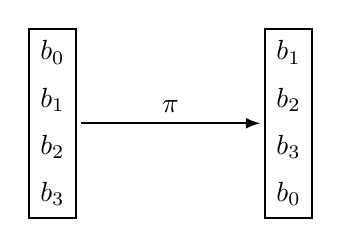
\begin{tikzpicture}[>=latex,thick]
\def\s{0.6}
\begin{scope}
\draw (0,0) rectangle (\s,{4*\s});
\foreach \y in {1,...,3}{
	\draw (0,{\y*\s}) (\s,{\y*\s});
}
\node at ({0.5*\s},{0.5*\s}) {$b_3$};
\node at ({0.5*\s},{1.5*\s}) {$b_2$};
\node at ({0.5*\s},{2.5*\s}) {$b_1$};
\node at ({0.5*\s},{3.5*\s}) {$b_0$};
\end{scope}
\draw[->] ({1.1*\s},{2*\s}) -- ({4.9*\s},{2*\s});
\node at ({3*\s},{2*\s}) [above] {$\pi$};
\begin{scope}[xshift=3cm]
\draw (0,0) rectangle (\s,{4*\s});
\foreach \y in {1,...,3}{
	\draw (0,{\y*\s}) (\s,{\y*\s});
}
\node at ({0.5*\s},{0.5*\s}) {$b_0$};
\node at ({0.5*\s},{1.5*\s}) {$b_3$};
\node at ({0.5*\s},{2.5*\s}) {$b_2$};
\node at ({0.5*\s},{3.5*\s}) {$b_1$};
\end{scope}
\end{tikzpicture}
\end{center}
\item
Die $S$-Operation wendet die $S$-Box auf jedes Byte eines Vektors an.
\item
Die $r_i$ Operation addiert in Runde $i$ eine Konstante $r_i$ zur
$0$-Komponente.
\end{itemize}
Die Konstante $r_i$ ist wieder ein einzelnes Byte und es ist daher
naheliegend, diese Bytes mit Hilfe der Arithmetik in $\mathbb{F}_{2^8}$
zu erzeugen.
Man kann daher $r_i$ definieren als
$(\texttt{02}_{16})^{i-1}\in\mathbb{F}_{2^8}$.

\subsection{Runden}
Der AES-Verschlüsselungsalgorithmus besteht jetzt darin, die bisher
definierten Operationen wiederholt anzuwenden.
Eine einzelne Runde besteht dabei aus folgenden Schritten:
\begin{enumerate}
\item Wende die $S$-Box auf alle Bytes des Blocks an.
\item Führe den Zeilenshift durch.
\item Mische die Spalten (wird in der letzten Runde)
\item Erzeuge den nächsten Rundenschlüssel
\item Addiere den Rundenschlüssel
\end{enumerate}
Der AES-Verschlüsselungsalgorithmus beginnt damit, dass der Schlüssel
zum Datenblock addiert wird.
Anschliessend werden je nach Blocklänge verschiedene Anzahlen von
Runden durchgeführt, 10 Runden für 128\,bit, 12 Runden für 192\,bit und
14 Runden für 256\,bit.






%\input{chapters/90-crypto/rs.tex}

\section*{Übungsaufgaben}
\rhead{Übungsaufgaben}
\aufgabetoplevel{chapters/90-crypto/uebungsaufgaben}
\begin{uebungsaufgaben}
\uebungsaufgabe{9001}
\end{uebungsaufgaben}

